\documentclass[11pt,a4paper]{jarticle}
\usepackage[dvipdfmx]{graphicx}
\usepackage{url}

\renewcommand{\baselinestretch}{1.05} 
\marginparwidth=0cm
\topmargin=-1cm
\headheight=0.3cm
\headsep=0.7cm
\oddsidemargin=0cm
\evensidemargin=0cm
%\textwidth=43zw
\textwidth=15.92cm
%\textheight=43.3\baselineskip
\baselineskip = 0.5744cm
\textheight=43\baselineskip

\itemsep=0.05\baselineskip
\parsep=0pt
\topsep=0.01\baselineskip
\partopsep=0pt
\listparindent=0zw

%% header and footer
\usepackage{fancyhdr}
\pagestyle{fancy}
\lhead{2017年度 春学期授業}
\chead{インタラクティブ・アート実習}
\rhead{担当教員: 松下 光範}
\cfoot{\thepage}
\renewcommand{\headrulewidth}{0pt}
\renewcommand{\footrulewidth}{0pt}

\usepackage{ascmac}
\usepackage{listings,jlisting}
\usepackage{color}
\definecolor{OliveGreen}{cmyk}{0.64,0,0.95,0.40}
\definecolor{colFunc}{rgb}{1,0.07,0.54}
\definecolor{CadetBlue}{cmyk}{0.62,0.57,0.23,0}
\definecolor{Brown}{cmyk}{0,0.81,1,0.60}
\definecolor{colID}{rgb}{0.63,0.44,0}
\definecolor{rulesepcolor}{gray}{0.666}
\lstset{
  language=Java,%プログラミング言語によって変える。
  basicstyle={\ttfamily\small},
  keywordstyle={\color{OliveGreen}},
  %[2][3]はプログラミング言語によってあったり、なかったり
  keywordstyle={[2]\color{colFunc}},
  keywordstyle={[3]\color{CadetBlue}},%
  commentstyle={\color{Brown}},
  %identifierstyle={\color{colID}},
  stringstyle=\color{blue},
  tabsize=2,
  %frame=trBL,
  %numbers=left,
  numberstyle={\ttfamily\small},
  breaklines=true,%折り返し
  %backgroundcolor={\color[gray]{.95}},
  framexleftmargin=0mm,
  frame=single,
  rulesepcolor=\color{rulesepcolor},
  captionpos=b
}


%%%%%%%%%%%%%%%%%%%%%%%%%%%%%%%%%%%%%%%%%%%%%%%%%%%%%%%%%%%%%%%%
\begin{document}

% title
\section*{\LARGE{番外編 Firmataのインストール}}
%Arduinoには「Firmata」と呼ばれる、ArduinoなどのマイコンとPCとのコミュニケーションを行うプロトコルがあります。
%%%%%%%%%%%%%%%%%%%%%%%%%%%%%%%%%%%%%%%%%%%%%%%%%%%%%%%%%%%%%%%%

\section{Arduinoを使えるようにする手順}
\subsection{Standard Firmata を開く}
\begin{itemize}
\item ファイル → スケッチの例 → Firmata → StandardFirmata
\end{itemize}

 \begin{figure}[h]
 \centering
 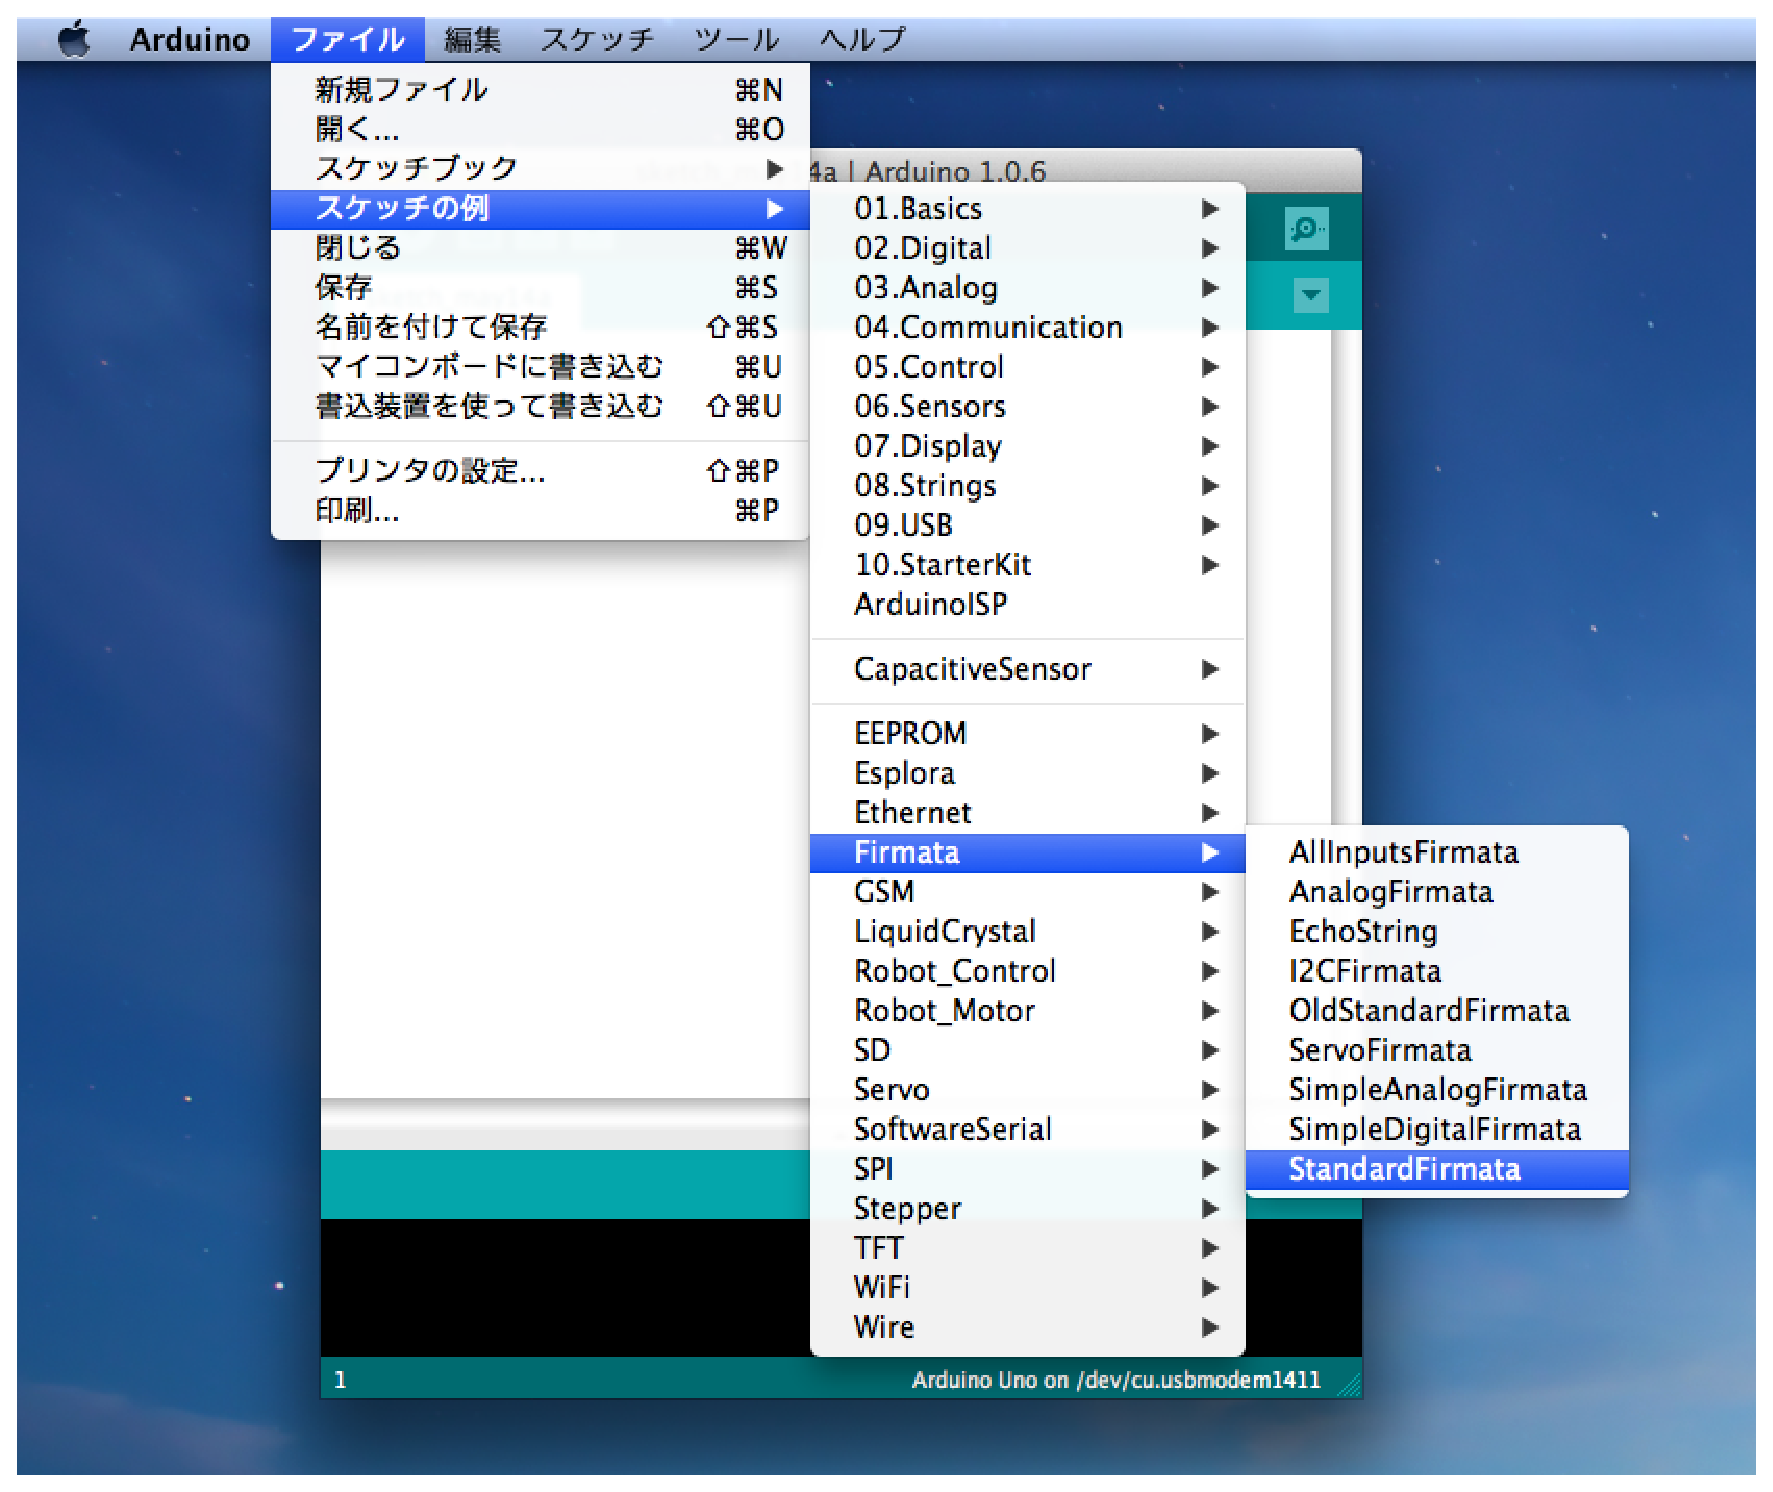
\includegraphics[width=0.63\columnwidth]{img/firmata3.eps}
\end{figure}

\subsection{シリアルポートの確認}
\begin{itemize}
\item ツール → シリアルポート → 「/dev/tty.usbmodem$\cdots$」から始まるポートを選択する
\end{itemize}

 \begin{figure}[h]
 \centering
 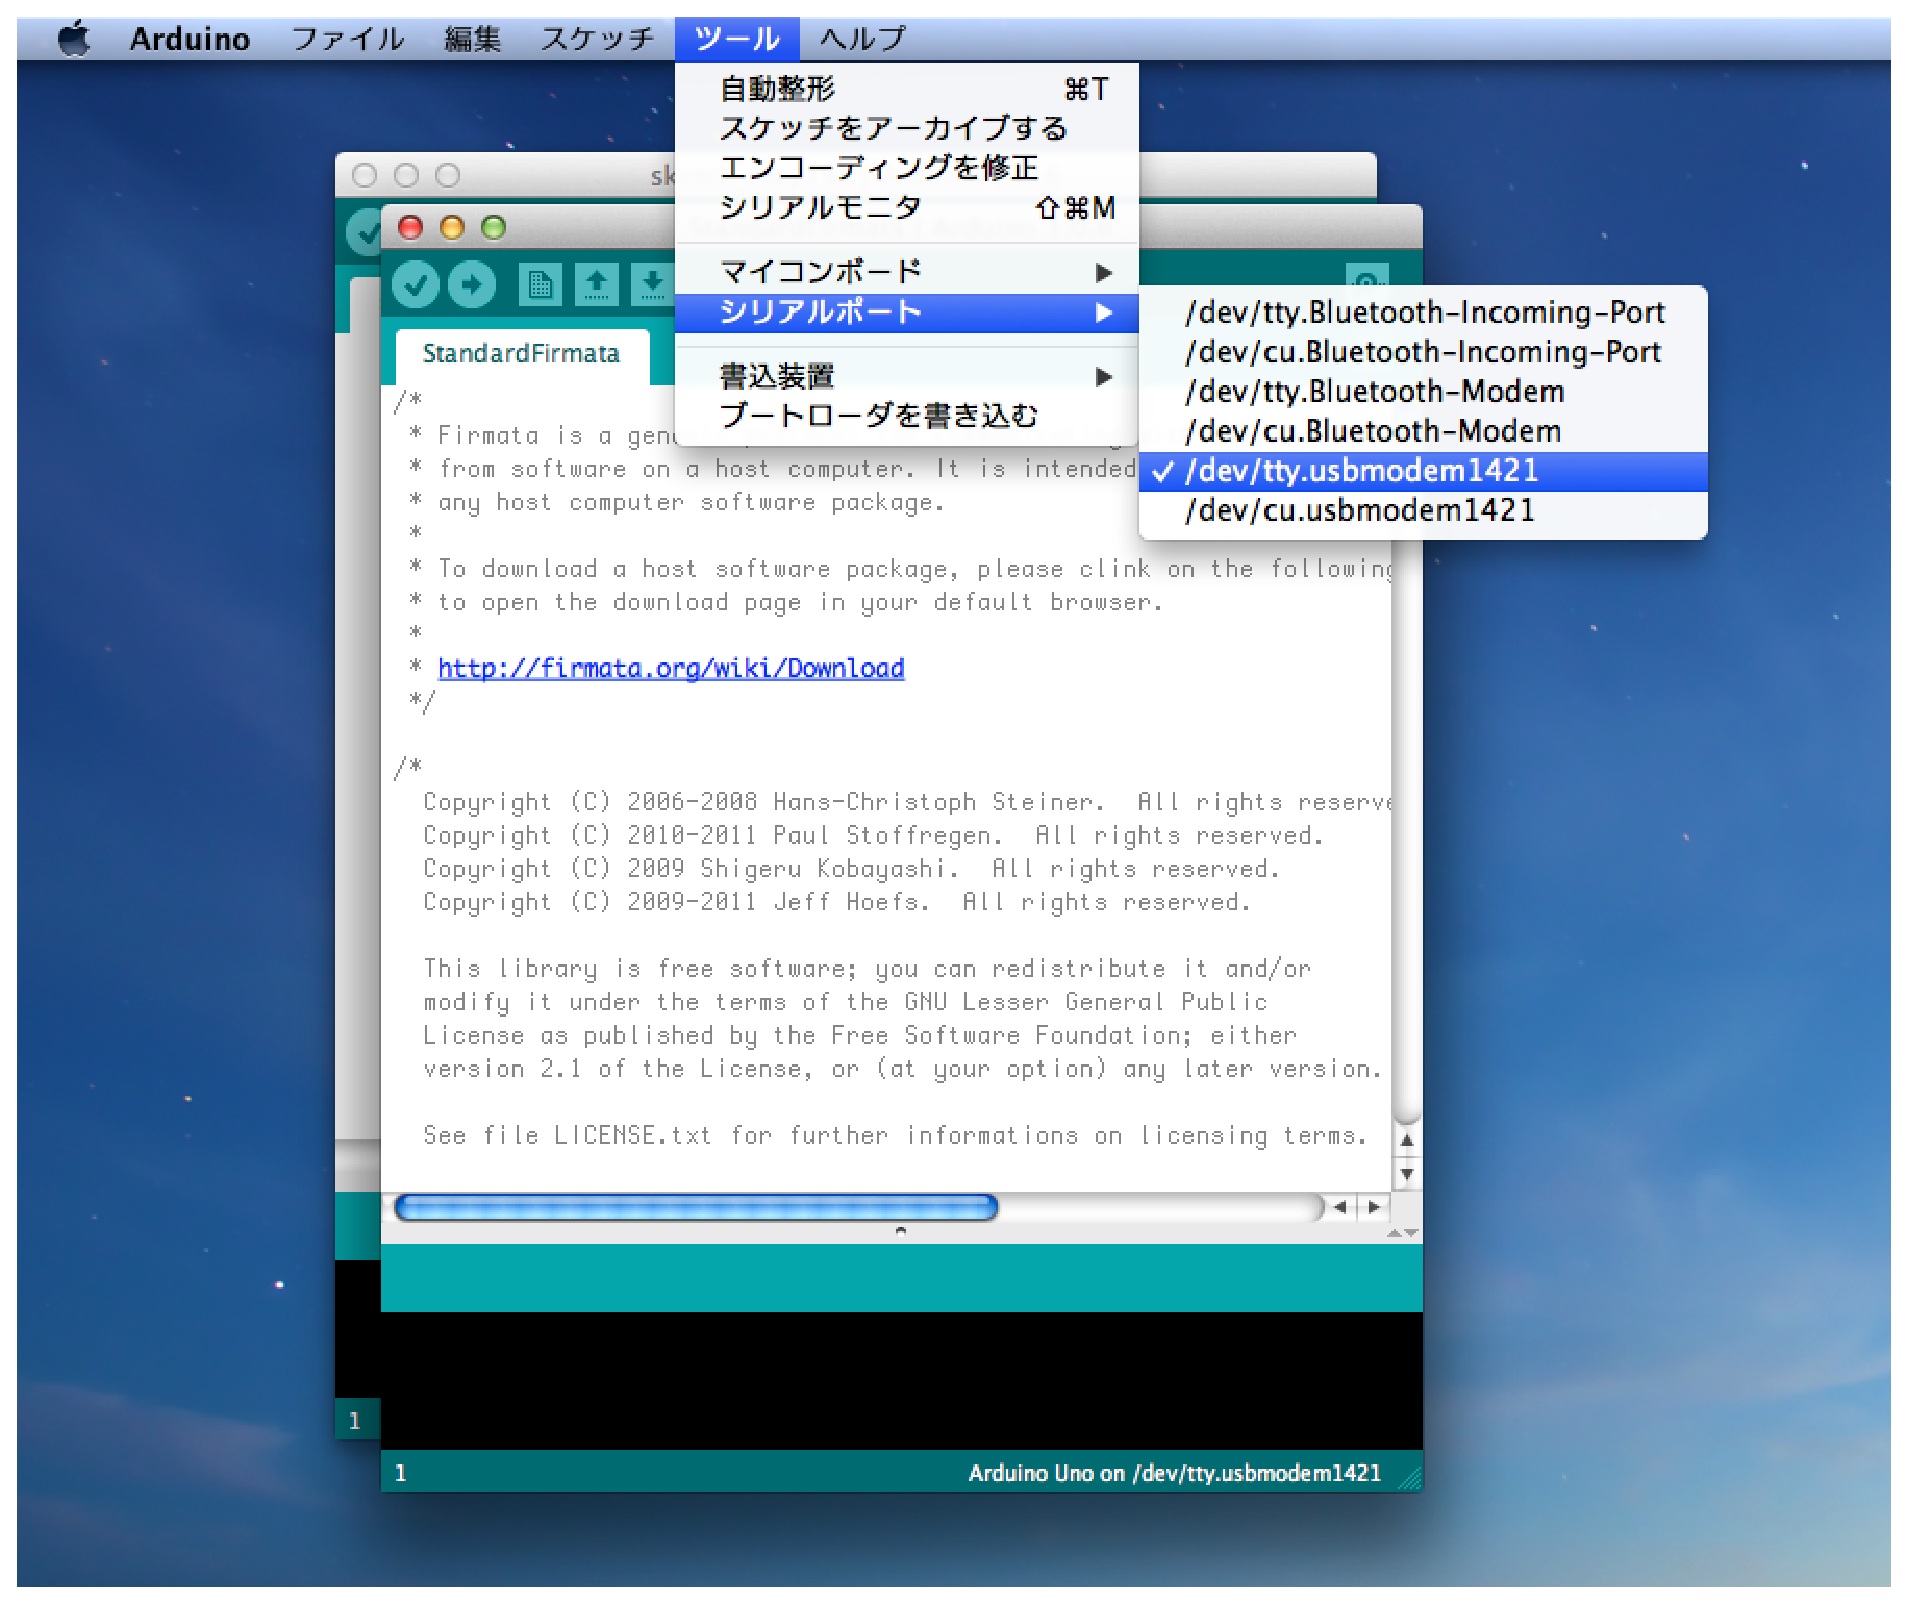
\includegraphics[width=0.63\columnwidth]{img/firmata5.eps}
\end{figure}

\newpage

\subsection{Arduionoに書き込む}
\begin{itemize}
\item 「マイコンボードに書き込む」ボタンをクリック
\end{itemize}

 \begin{figure}[h]
 \centering
 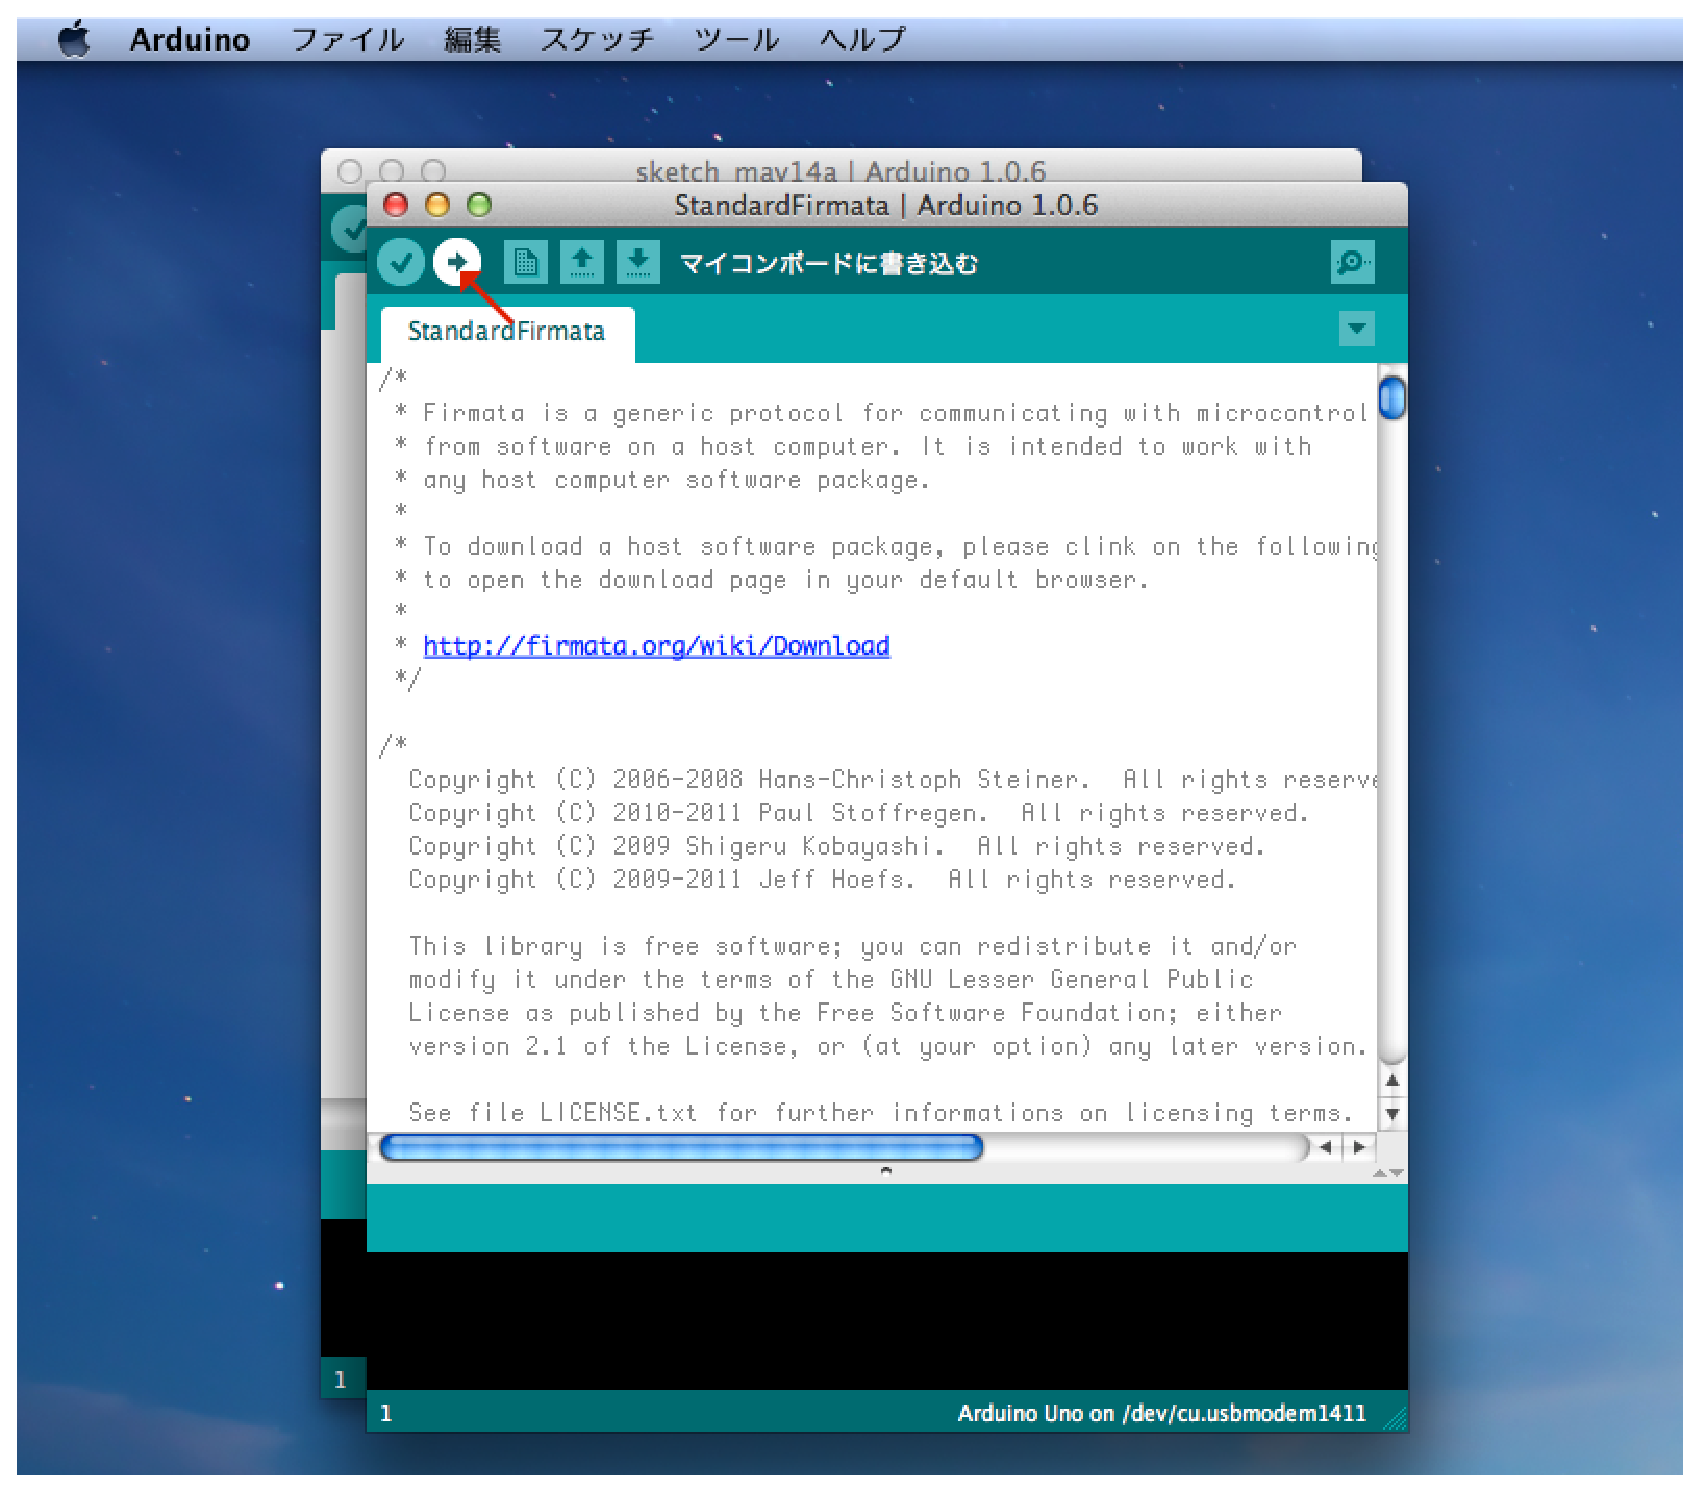
\includegraphics[width=0.63\columnwidth]{img/firmata6.eps}
\end{figure}

この操作が完了したら、手持ちのPCでArduinoが使えるようになります。


%\subsection*{回路}
%\begin{figure}[h!]
% \begin{minipage}{0.5\columnwidth}
%  \centering
%  \includegraphics[width=0.7\columnwidth]{img/}
 % \begin{center}
%   \textbf{赤外線センサ}
 % \end{center}
% \end{minipage}
% \begin{minipage}{0.5\columnwidth}
%  \centering
%  \includegraphics[width=\columnwidth]{img/}
%  \begin{center}
%   \textbf{赤外線センサを用いた回路図}
%  \end{center}
% \end{minipage}
%\end{figure}



%\begin{figure}[h!]
% \begin{minipage}{0.32\columnwidth}
%  \centering
%%  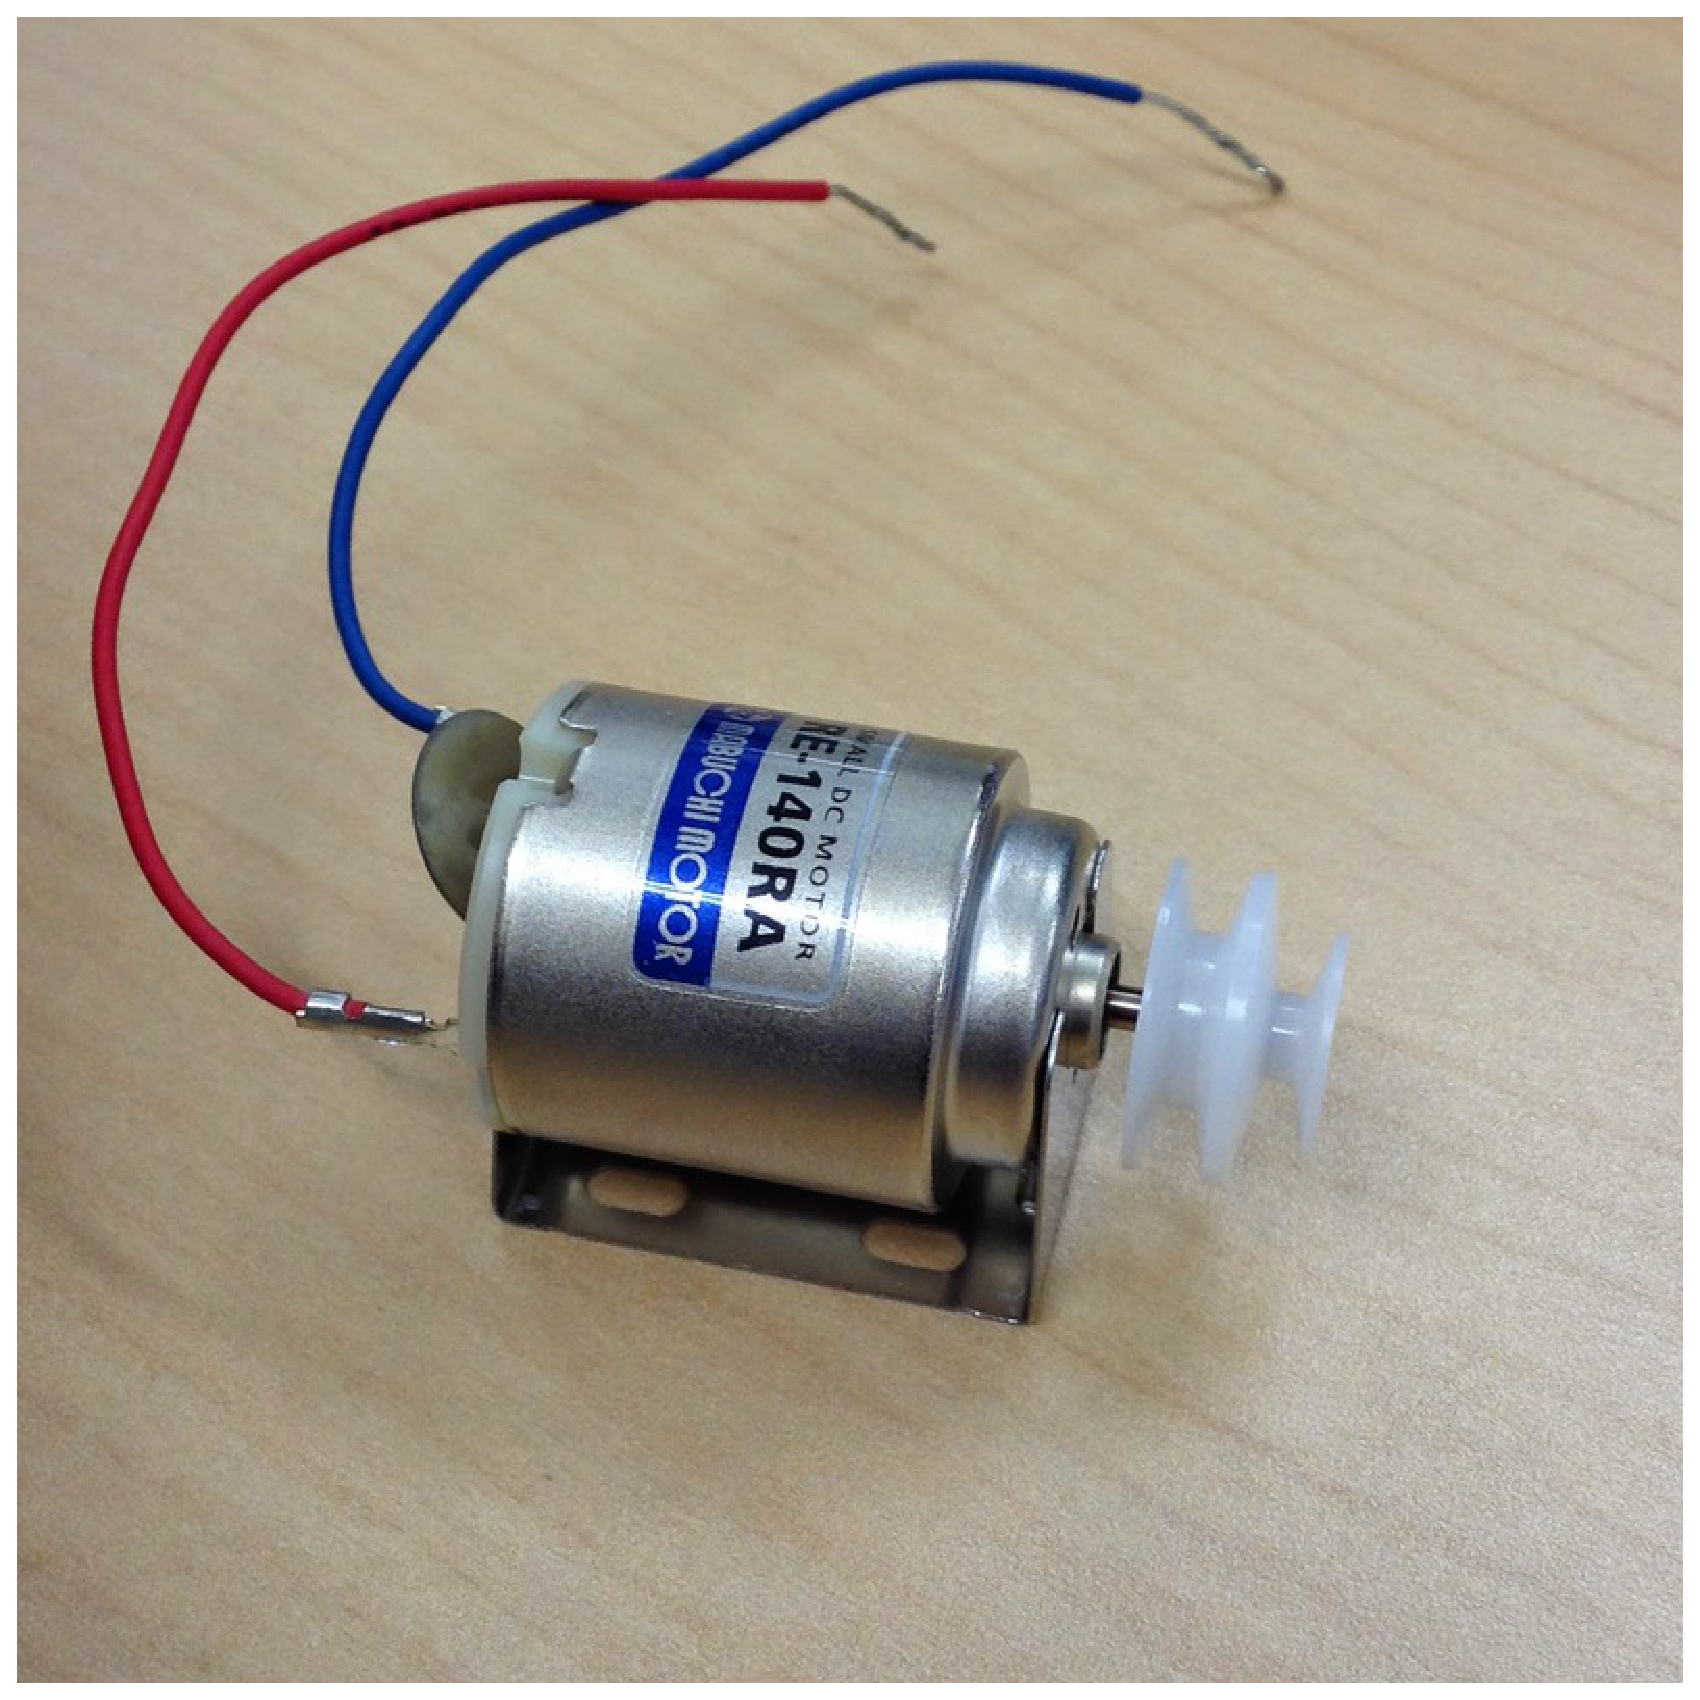
\includegraphics[width=\columnwidth]{img/motor.eps}
%  \begin{center}
%   \textbf{モーター(RE-140RA)}
%  \end{center}
% \end{minipage}
% \begin{minipage}{0.32\columnwidth}
%  \centering
%  %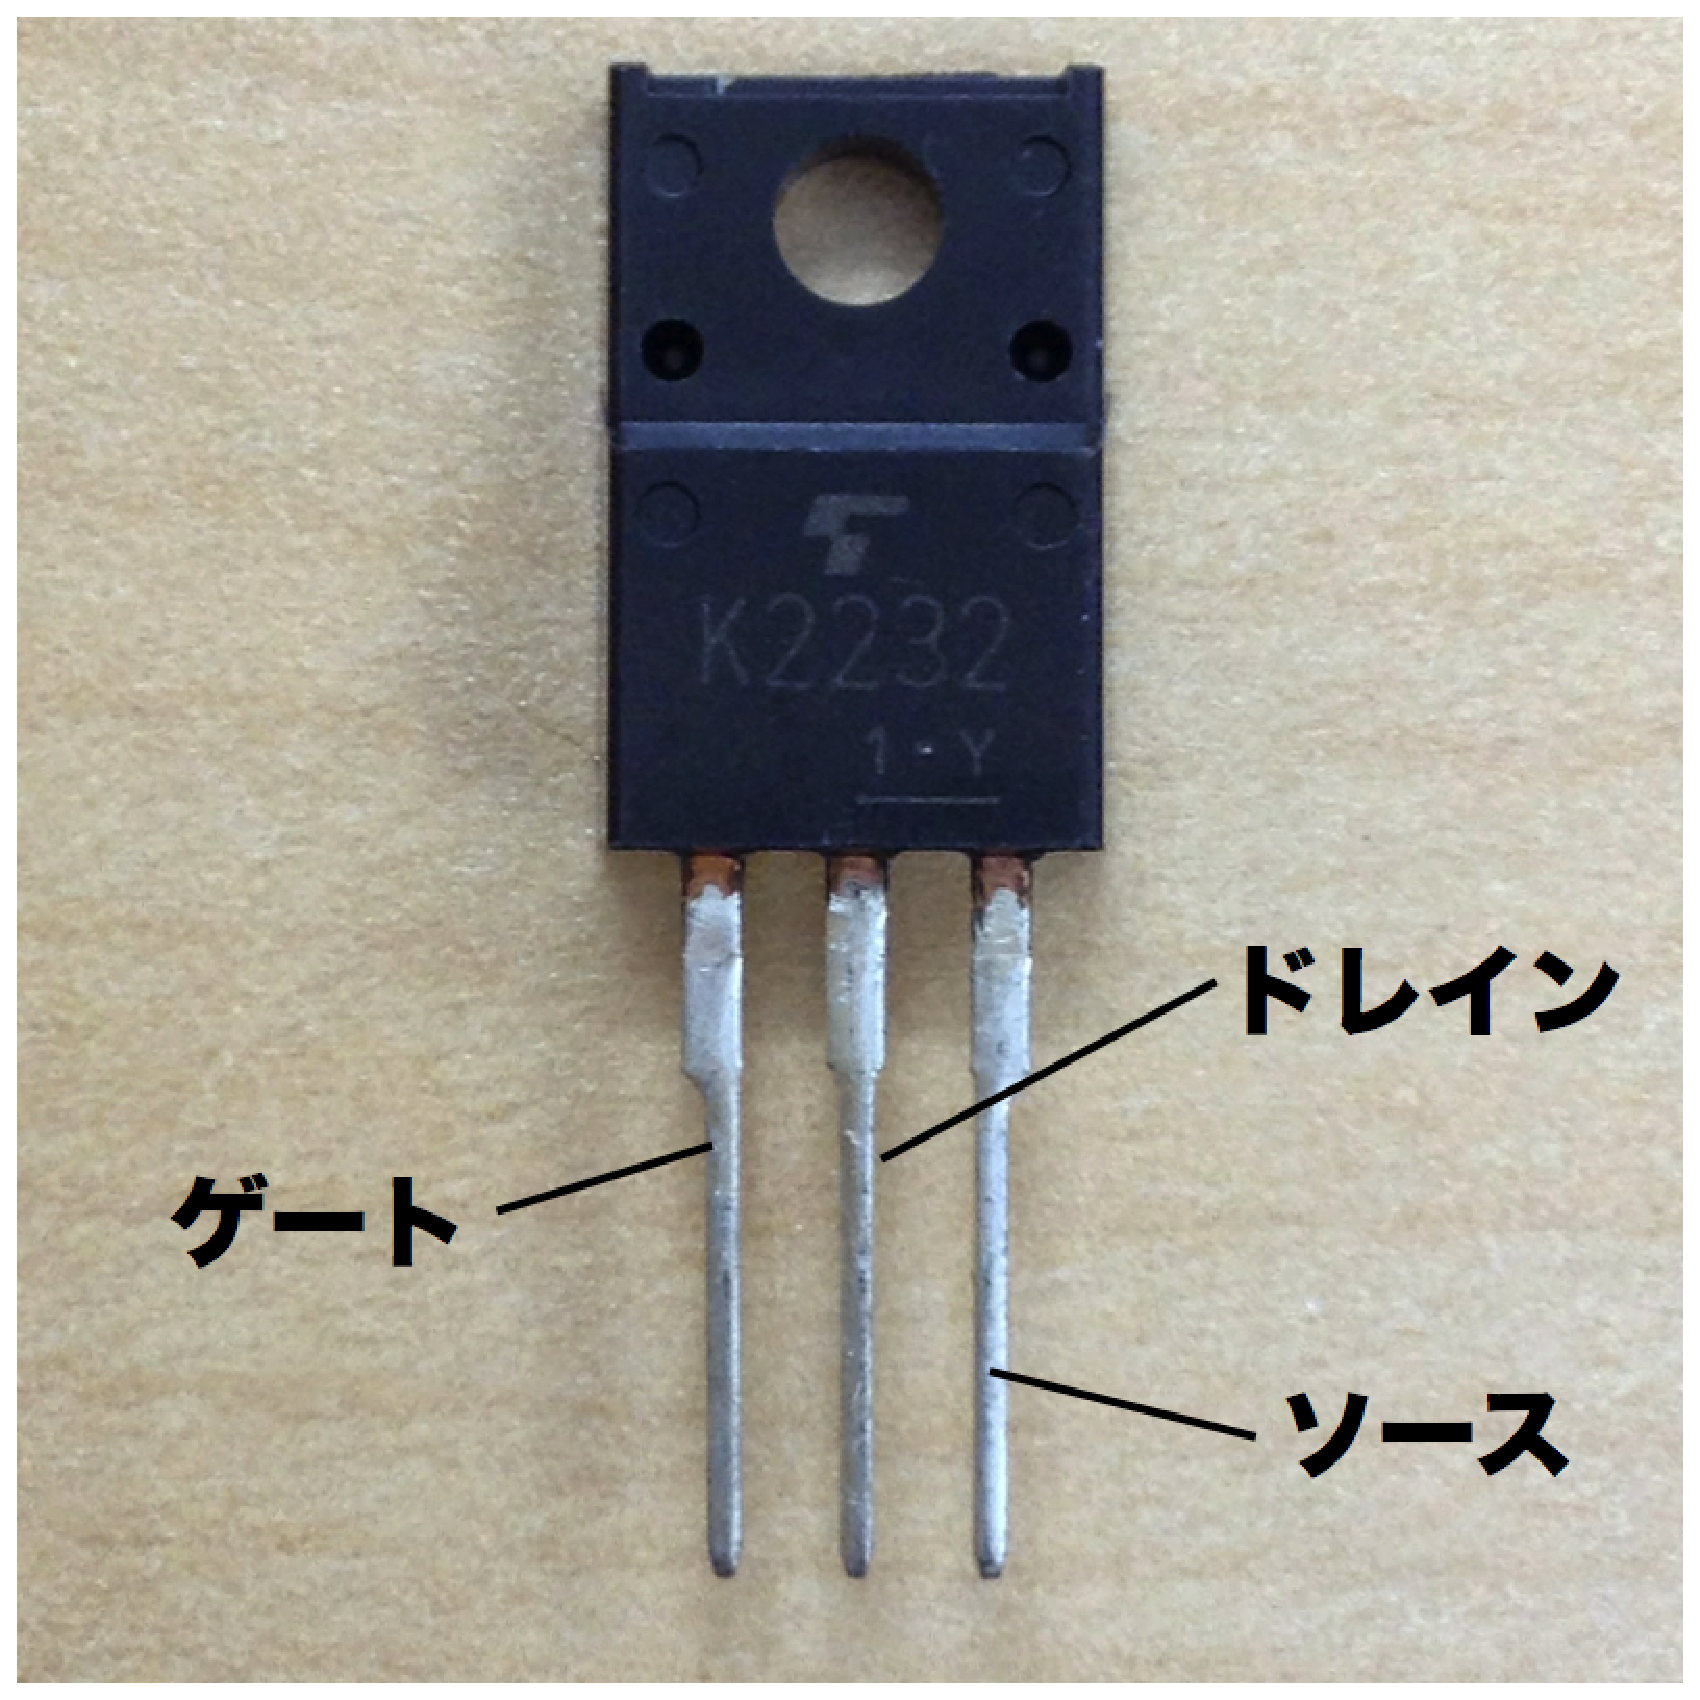
\includegraphics[width=\columnwidth]{img/fet.eps}
%  \begin{center}
%   \textbf{FET (2SK2232)}
%  \end{center}
% \end{minipage}
% \begin{minipage}{0.32\columnwidth}
%  \centering
%%  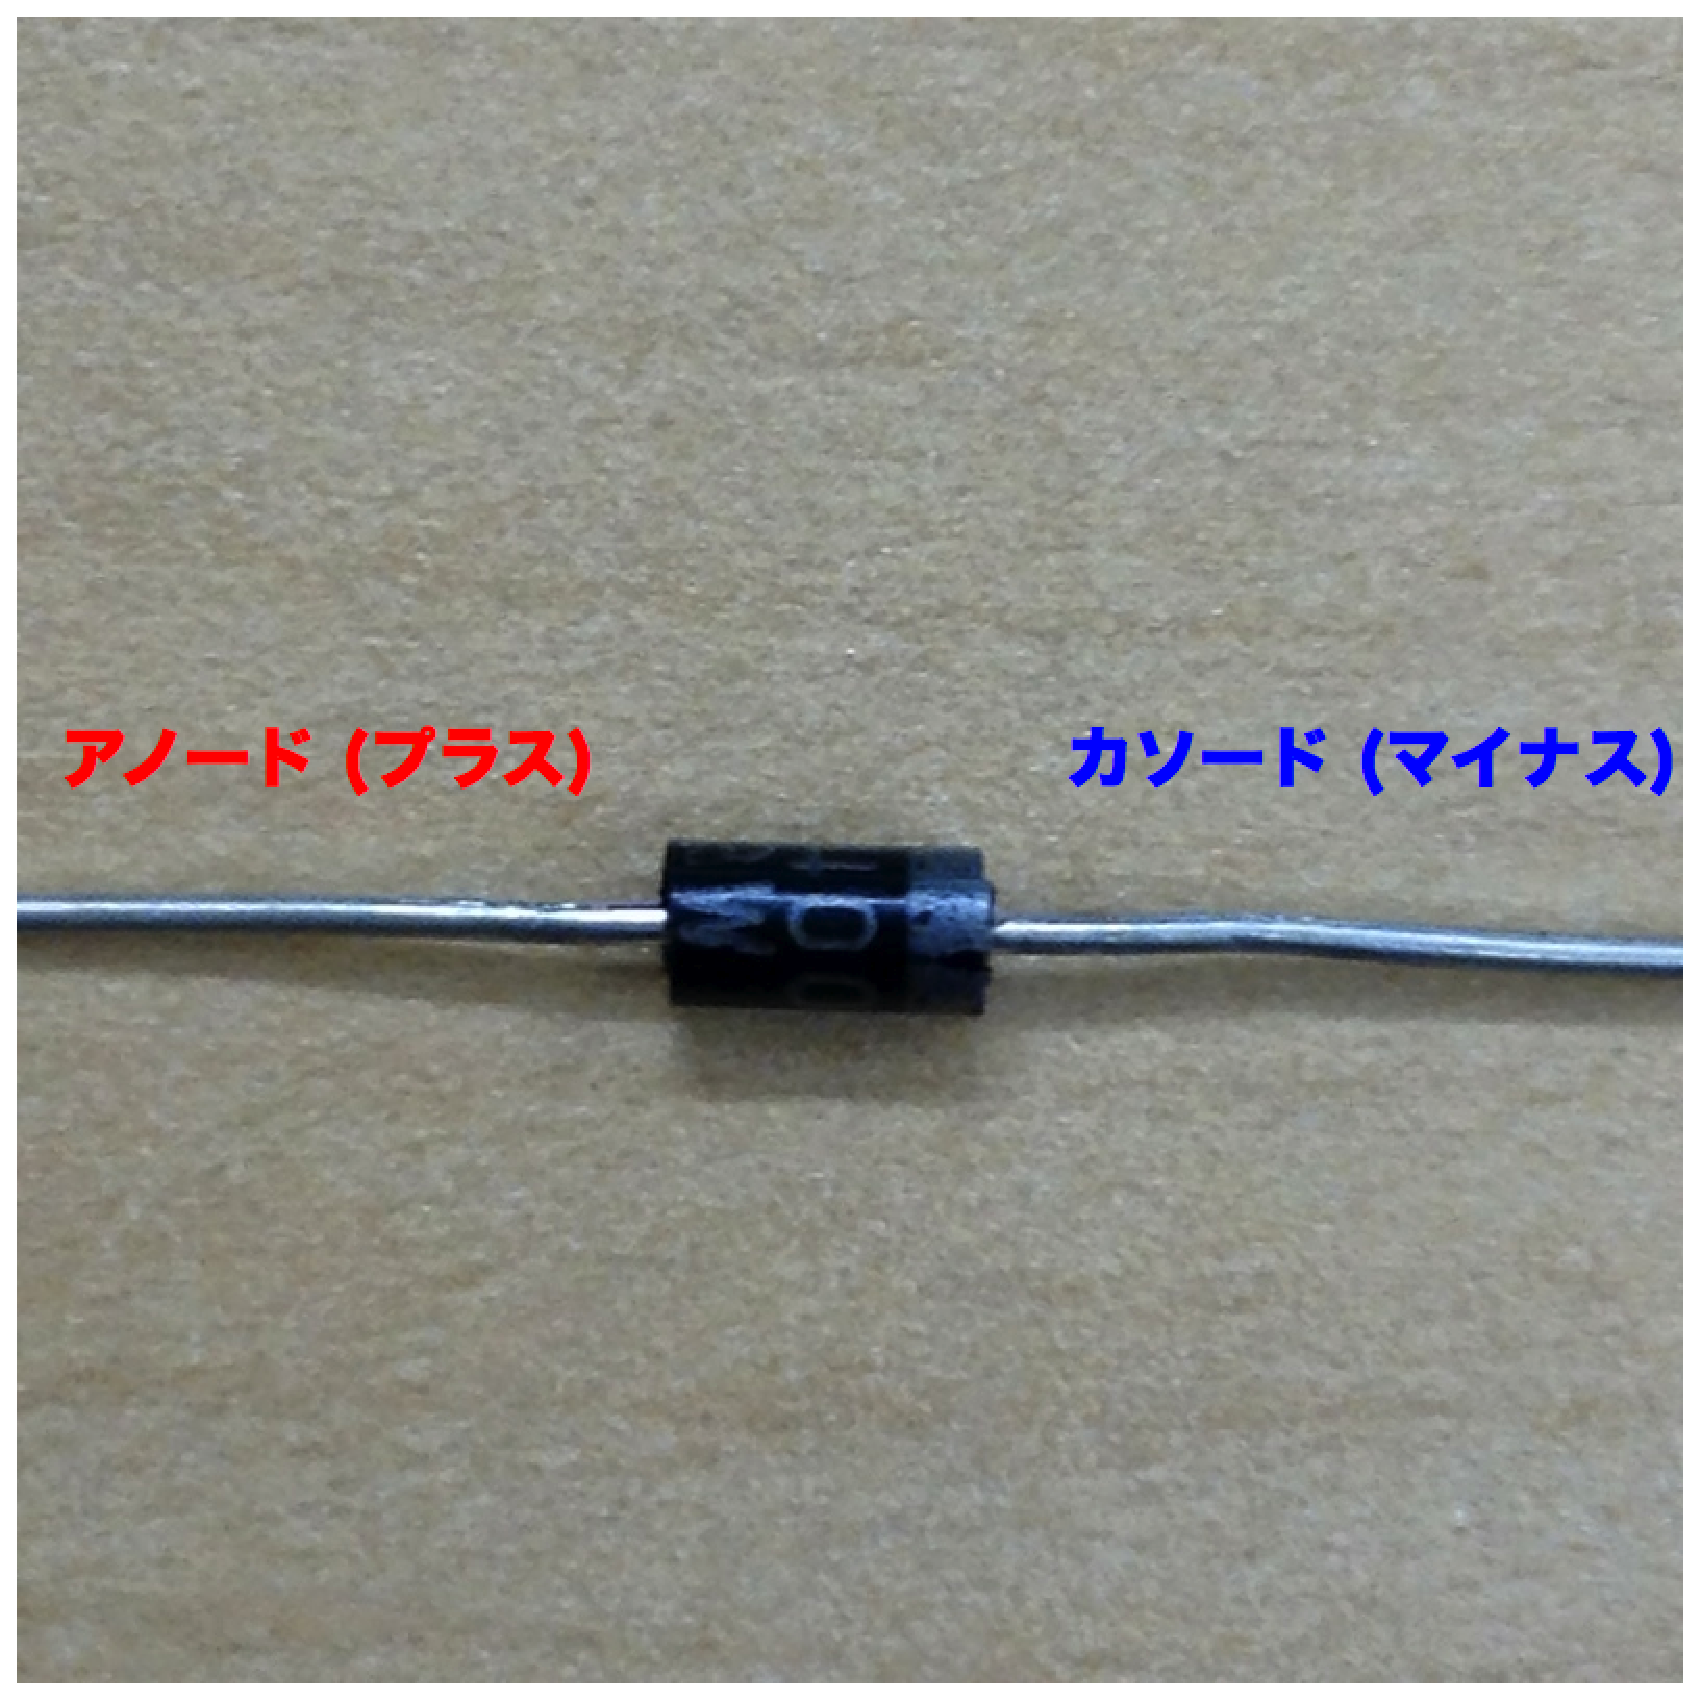
\includegraphics[width=\columnwidth]{img/diode.eps}
%  \begin{center}
%   \textbf{ダイオード}
%  \end{center}
% \end{minipage}
%\end{figure}


%\subsection*{回路}
%\begin{figure}[h!]
% \centering
% %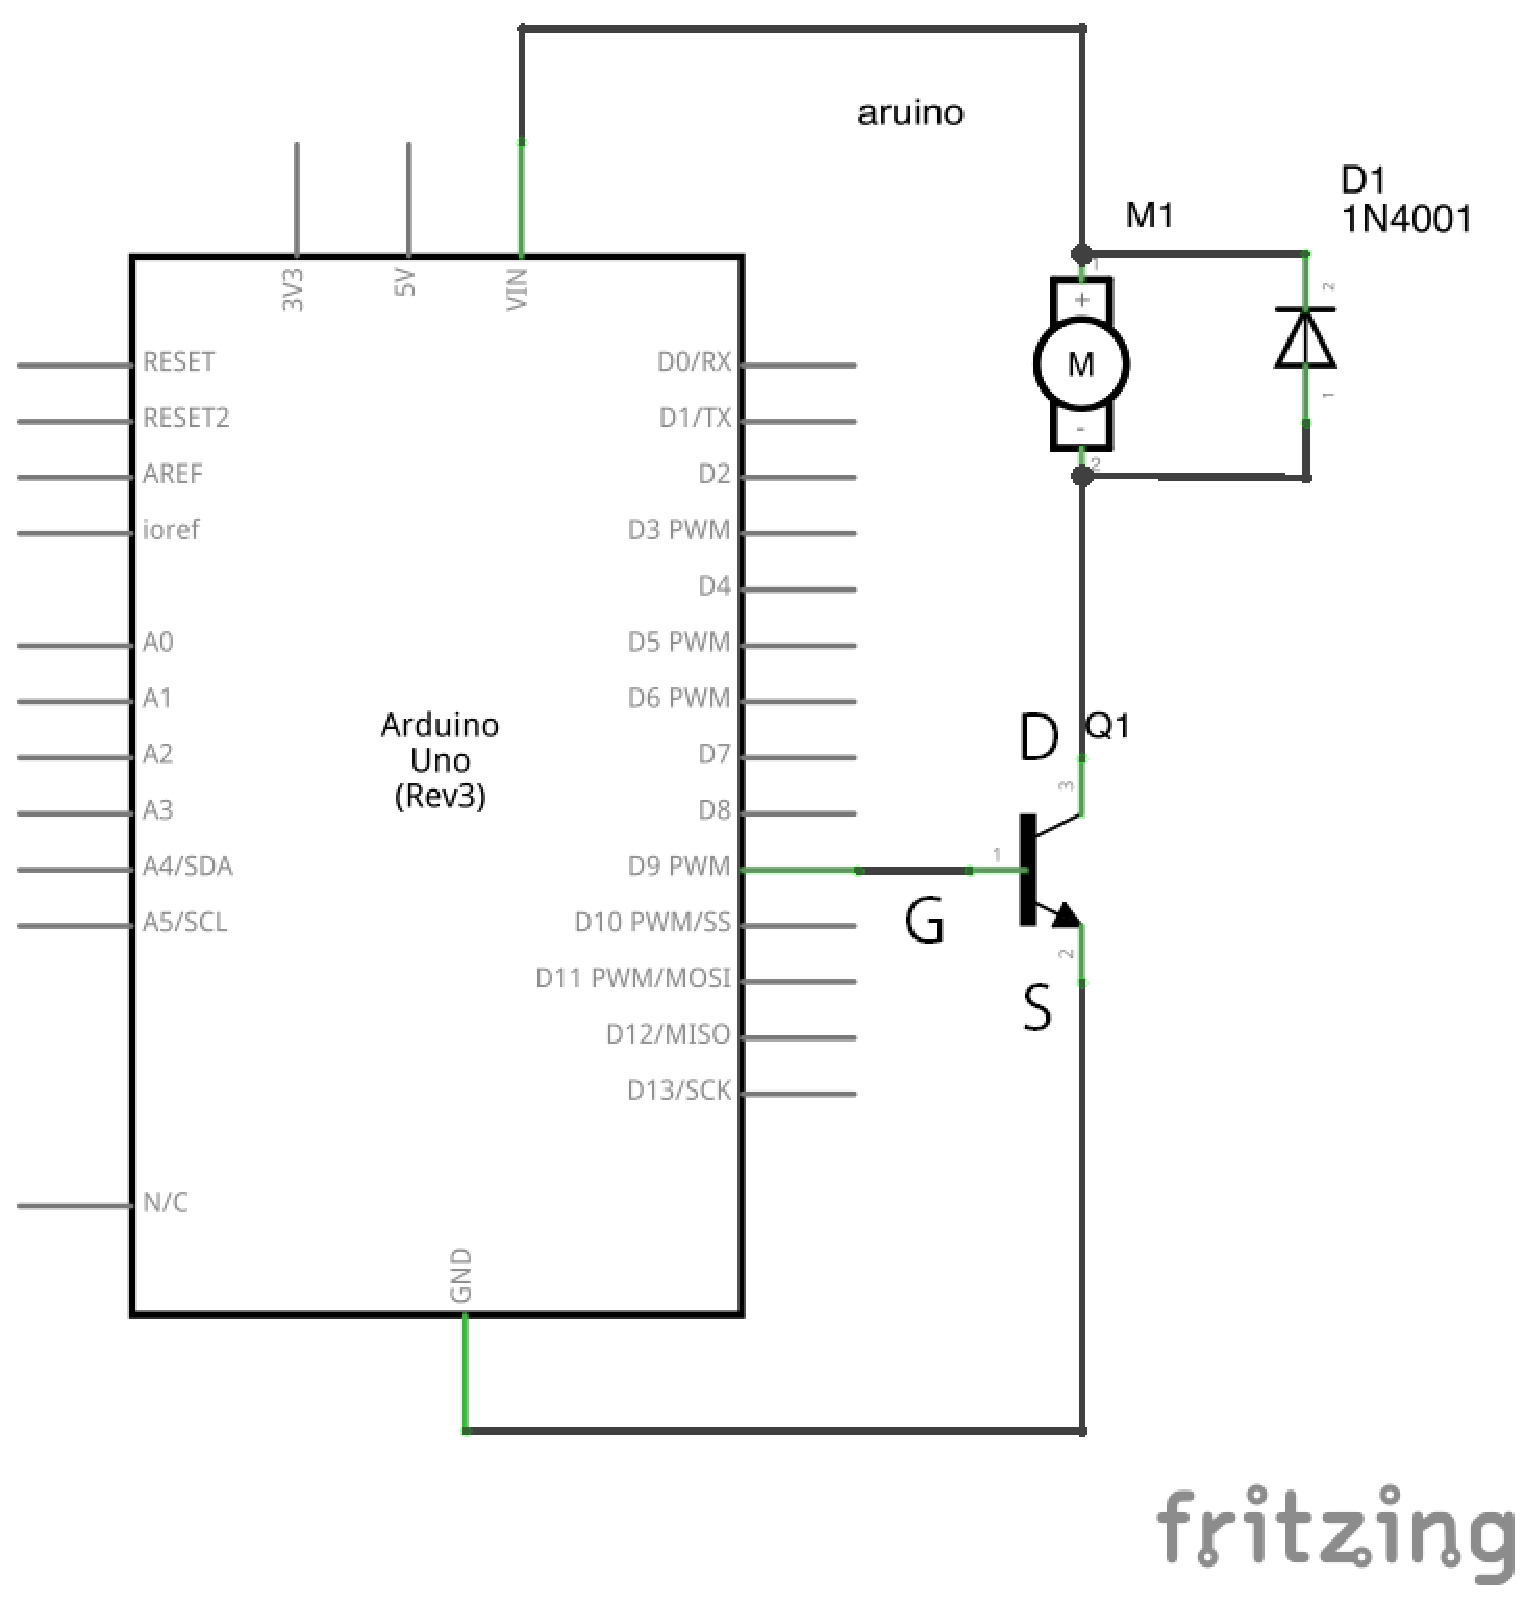
\includegraphics[width=0.5\columnwidth]{img/motor_control_circuit.eps}
% \begin{center}
%  \textbf{モーター制御のための回路図}
% \end{center}
%\end{figure}



\end{document}